
\subsection{SEIS2VIEWER, Plotting hypocentres in 3D}
\label{subs:seis2viewer}
\label{page:seis2viewer}

The program is written by \textbf{Ruben Soares Lu\'is} (ruben.so.luis@gmail.com) and use 
the SeismicityViewer50 program by \textbf{Anthony Lomax}. To program has been aliased to smap.

\index{SEIS2VIEWER}

\textbf{Overview}

seis2viewer is a wrapper for the application SeismicityViewer, developed by Anthony Lomax for rapid mapping of seismic events. SeismicityViewer displays hypocenter locations in 3D as well as station locations and P/S residuals. Geographic and geologic features can also be displayed as well as focal mechanisms. Please find details here:\newline
\url{http://alomax.free.fr/seismicity/}

seis2viewer has been created to take information from a nordic file from Seisan and convert it in a format usable by SeismicityViewer 5.0 (NLLoc Format). It automatically launches Seismicity Viewer, generating a set of files required for its operation.

In its current version, seis2viewer allows the visualization of hypocenters and magnitudes in SeismicityViewer 5.0. Other information, such as station locations, P and S residuals, etc. is not displayed.


\textbf{Installation and Configuration}

\begin{enumerate}
\item[1:] \textbf{Configuration Files:}

\begin{itemize}
\item \texttt{seis2viewer.def} (mandatory): seis2viewer uses a \textbf{single} configuration file: \texttt{seis2viewer.def}, which may contain references to other files containing information on maps, elevation, localities, etc. The file \texttt{seis2viewer.def} is actually passed directly to Seismicity Viewer adding only a reference to an automatically created file. This operation is transparent to the user. As such, the configurations can be obtained from the Seismicity Viewer 5.0 website: \url{http://alomax.free.fr/seismicity/}
\item Other files: \texttt{seis2viewer.def} may reference other files containing map information, elevation data, locality names, etc. These files should follow the definitions presented in the Seismicity Viewer 5.0 website.
\end{itemize}


\item[2:] \textbf{Installation}

seis2viewer is distributed as a single .jar file (\texttt{seis2viewer.jar}), containing all the necessary classes to work, including Seismicity Viewer 5.0. This file should be placed in the PRO directory of seisan.
To facilitate the usage of seis2viewer, the administrator should create an executable script file to call seis2viewer. As an example, the executable script should contain the following line:

\begin{verbatim}
java -jar $SEISAN_TOP/PRO/seis2viewer.jar $1        (for unix/linux)
java -jar %SEISAN_TOP%/PRO/seis2viewer.jar %1%      (for windows)
\end{verbatim}

The configuration file, \texttt{seis2viewer.def}, and any other required files should be placed in the DAT directory of seisan. Alternatively, the user may have its configurations on the working directory.

\item[2:] \textbf{Automatically Generated Files}
seis2viewer generates a set of files to be used by Seismicity Viewer 5.0. Although these files are, in principle, irrelevant to the user, it is nevertheless important to mention them for reference purposes.

\begin{itemize}
\item \texttt{seismicitydefaults}: This is the default configuration file for Seismicity Viewer. It contains a reference to the converted events file, \texttt{seis2viewer.hyp}.
\item \texttt{seis2viewer.hyp}: This file contains a translation of the event file selected by the user for visualization in NonLinLoc format, appropriate for Seismicity Viewer.
\item \texttt{seis2viewer.hdr}: This is an automatically generated grid file for the area surrounding the events to be visualized. It is only created if the maximum distance in longitude or latitude between events is less than 20 degrees.
\end{itemize}

\end{enumerate}

\textbf{Usage}

seis2viewer can be used directly with a nordic file containing one or more events (e.g. \texttt{select.out}) as:

\begin{verbatim}
java -jar %SEISAN_TOP%/PRO/seis2viewer.jar select.out    (windows)
java -jar $SEISAN_TOP/PRO/seis2viewer.jar select.out     (unix/linux)
\end{verbatim}

or, if the executable script has been created, as (assuming the script is called '\texttt{smap}')\newline
\texttt{smap select.out}\newline
seis2viewer can also be called directly from eev, as an external program, using the prefix 'o' as:\newline
\texttt{osmap}\newline
In this case, smap will try to find the file eev.cur.out, which is automatically generated by eev and contains a reference to the event that is currently under work.


%SEIS2VIEWER can run in two modes: 
%
%One earthquake from EEV:\newline
%Type \texttt{osmap eev.cur.sfile} in EEV.
%
%Many earthquakes:\newline
%Type e.g. \texttt{smap collect.out} to 
%plot many earthquakes from file collect.out. Note if the earthquakes cover a large area 
%they will be shown in Global mode, if the earthquakes 
%cover a small area they will be shown in Local mode.
%The depth of the earthquakes can only be shown in Local mode.
%
\begin{figure}
\htmlimage{scale=2.0}
\centerline{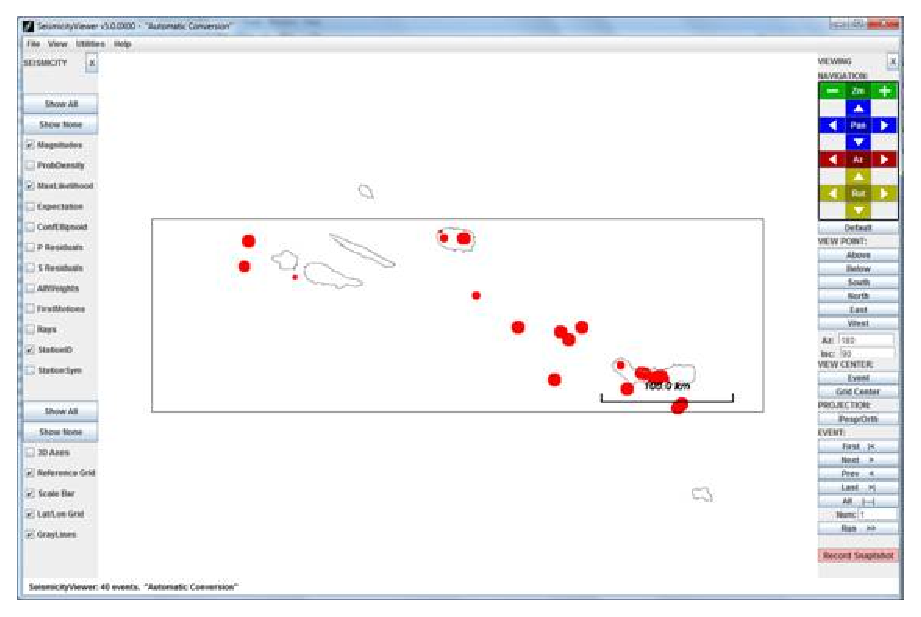
\includegraphics[width=0.9\linewidth]{fig/seis2viewer}}
\caption{Epicenter map by SEIS2VIEWER.}
\label{fig:seis2viewer}
\end{figure}

%SEIS2VIEWER uses the following files from the 
%\textbf{DAT} folder:
%\textbf{seis2viewer.def}, and one of the coast line files 
%\textbf{azores.xyz} or
%\textbf{europe.xyz}.
%Note: it seesm like the file azores.xyz is only found if in working directory.
%You can construct your own coast line files, e.g. using GMT in unix by:
%
%\begin{verbatim}
%pscoast -M -W1 -P -R-60.00/50.0/60/78r -JT-40/10 -Dl > greenland.xy
%awk '{print $0" 0"}' greenland.xy > greenland.tmp
%grep -v "# Data" greenland.tmp | sed 's/>\([a-z]*\).*/> GMT_LONLATELEV_M/' > greenland.xyz
%\end{verbatim}


